\chapter{Benchmarking Results}

\section{Results of the Compression Benchmark}
\label{app:compression:results}

This appendix provides tables containing the results of the benchmarks that
have been performed for comparing the indexing and querying performance of the
index structure with various compression algorithms.
Tables~\ref{tab:indexing-performance} have been used for generating the charts
from Section~\ref{sec:compression:indexing-performance}.
Tables~\ref{tab:query-time} have been used for generating the charts from
Section~\ref{sec:compression:query-performance}.

\begin{table*}[h!]
	\centering
	\ra{1.3}
	\resizebox{0.8\linewidth}{!}{%
	\subfloat[Wikipedia]{%
	\begin{tabular}{@{}rcr@{\hs}rcr@{\hs}r@{\hs}r@{\hs}r@{\hs}}
	\toprule
	& \phantom{a} 
	& \multicolumn{2}{c}{Time (s)} 
	& \phantom{a} 
	& \multicolumn{4}{c}{Sizes (GB)} \\ 
	\cmidrule{3-4} \cmidrule{6-9}
	Method && Total & Opt && Doc & Frq & Pos & Total \\
	\midrule
	AFOR-1 && 410 & 114&& 0.353 & 0.109 & 0.698 & 1.160\\
	AFOR-2 && 409 & 128&& 0.340 & 0.093 & 0.655 & 1.088 \\
	FOR && 443 & 128&& 0.426 & 0.178 & 0.811 & 1.415\\
	PFOR && 438 & 127 && 0.428 & 0.106 & 0.745 & 1.279\\
	Rice && 492 & 228 && 0.332 & 0.061 & 0.600 & 0.993\\
	S9-64 && 462 & 124&& 0.356 & 0.103 & 0.662 & 1.121\\ 
	VByte && 433 & 132 && 0.402 & 0.291 & 0.714 & 1.407\\      
	\bottomrule
	\end{tabular}
	}\quad%
	\subfloat[Blog]{%
	\begin{tabular}{@{}rcr@{\hs}rcr@{\hs}r@{\hs}r@{\hs}r@{\hs}}
	\toprule
	& \phantom{a} 
	& \multicolumn{2}{c}{Time (s)} 
	& \phantom{a} 
	& \multicolumn{4}{c}{Sizes (GB)} \\ 
	\cmidrule{3-4} \cmidrule{6-9}
	Method && Total & Opt && Doc & Frq & Pos & Total \\
	\midrule
	AFOR-1 && 12337 & 4813&& 7.868 & 2.366 & 21.058 & 31.292 \\
	AFOR-2 && 13040 & 4571&& 7.387 & 2.016 & 19.492 & 28.895 \\
	FOR && 12741 & 5888&& 9.115 & 3.882 & 26.780 & 39.777 \\
	PFOR && 13972 & 5387&& 9.097 & 2.464 & 23.975 & 35.536 \\
	Rice && 14099 & 7127&& 7.145 & 1.546 & 18.160 & 26.851 \\
	S9-64 && 13152 & 5414 && 7.892 & 2.197 & 19.711 & 29.800 \\
	VByte && 12320 & 5092 && 8.630 & 5.610 & 22.063 & 36.303 \\
	\bottomrule
	\end{tabular}
	}}\quad%
	
	\subfloat[DBpedia]{%
	\resizebox{.3\linewidth}{!}{%
	\begin{tabular}{@{}rcr@{\hs}rcr@{\hs}r@{\hs}r@{\hs}r@{\hs}r@{\hs}r@{}}
	\toprule
	& \phantom{a} 
	& \multicolumn{2}{c}{Time (s)} 
	& \phantom{a} 
	& \multicolumn{6}{c}{Sizes (GB)} \\ 
	\cmidrule{3-4} \cmidrule{6-11}
	Method && Total & Opt && Ent & Frq & Att & Val & Pos & Total \\
	\midrule
	AFOR-1 && 536 & 139 && 0.246 & 0.043 & 0.141 & 0.065 & 0.180 & 0.816 \\
	AFOR-2 && 540 & 142 && 0.229 & 0.039 & 0.132 & 0.059 & 0.167 & 0.758 \\
	AFOR-3 && 562 & 158 && 0.229 & 0.031 & 0.131 & 0.054 & 0.159 & 0.736 \\
	FOR && 594 & 158 && 0.315 & 0.061 & 0.170 & 0.117 & 0.216 & 1.049 \\
	PFOR && 583 & 167 && 0.317 & 0.044 & 0.155 & 0.070 & 0.205 & 0.946 \\
	Rice && 612 & 239 && 0.240 & 0.029 & 0.115 & 0.057 & 0.152 & 0.708 \\
	S-64 && 558 & 162 && 0.249 & 0.041 & 0.133 & 0.062 & 0.171 & 0.791 \\
	VByte && 577 & 164 && 0.264 & 0.162 & 0.222 & 0.222 & 0.245 & 1.335 \\
	\bottomrule
	\end{tabular}
	}}\quad%
	\subfloat[Geonames]{%
	\resizebox{.3\linewidth}{!}{%
	\begin{tabular}{@{}rcr@{\hs}rcr@{\hs}r@{\hs}r@{\hs}r@{\hs}r@{\hs}r@{}}
	\toprule
	& \phantom{a} 
	& \multicolumn{2}{c}{Time (s)} 
	& \phantom{a} 
	& \multicolumn{6}{c}{Sizes (GB)} \\ 
	\cmidrule{3-4} \cmidrule{6-11}
	Method && Total & Opt && Ent & Frq & Att & Val & Pos & Total \\
	\midrule
	AFOR-1 && 729 & 114 && 0.129 & 0.023 & 0.058 & 0.025 & 0.025 & 0.318 \\
	AFOR-2 && 732 & 107 && 0.123 & 0.023 & 0.057 & 0.024 & 0.024 & 0.307 \\
	AFOR-3 && 724 & 103 && 0.114 & 0.006 & 0.056 & 0.016 & 0.008 & 0.256 \\
	FOR && 748 & 102 && 0.150 & 0.021 & 0.065 & 0.025 & 0.023 & 0.349 \\
	PFOR && 741 & 134 && 0.154 & 0.019 & 0.057 & 0.022 & 0.023 & 0.332 \\
	Rice && 787 & 183 && 0.133 & 0.019 & 0.063 & 0.029 & 0.021 & 0.327 \\
	S-64 && 740 & 123 && 0.147 & 0.021 & 0.058 & 0.023 & 0.023 & 0.329 \\
	VByte && 737 & 141 && 0.216 & 0.142 & 0.143 & 0.143 & 0.143 & 0.929 \\
	\bottomrule
	\end{tabular}
	}}\quad%
	\subfloat[Sindice]{%
	\resizebox{.3\linewidth}{!}{%
	\begin{tabular}{@{}rcr@{\hs}rcr@{\hs}r@{\hs}r@{\hs}r@{\hs}r@{\hs}r@{}}
	\toprule
	& \phantom{a} 
	& \multicolumn{2}{c}{Time (s)} 
	& \phantom{a} 
	& \multicolumn{6}{c}{Sizes (GB)} \\ 
	\cmidrule{3-4} \cmidrule{6-11}
	Method && Total & Opt && Ent & Frq & Att & Val & Pos & Total \\
	\midrule
	AFOR-1 && 13734 & 1816 && 2.578 & 0.395 & 0.942 & 0.665 & 1.014 & 6.537 \\
	AFOR-2 && 13975 & 1900 && 2.361 & 0.380 & 0.908 & 0.619 & 0.906 & 6.082 \\
	AFOR-3 && 13847 & 1656 && 2.297 & 0.176 & 0.876 & 0.530 & 0.722 & 5.475 \\
	FOR && 14978 & 1749 && 3.506 & 0.506 & 1.121 & 0.916 & 1.440 & 8.611 \\
	PFOR && 14839 & 2396 && 3.221 & 0.374 & 1.153 & 0.795 & 1.227 & 7.924 \\
	Rice && 15571 & 3281 && 2.721 & 0.314 & 0.958 & 0.714 & 0.941 & 6.605 \\
	S-64 && 14107 & 2163 && 2.581 & 0.370 & 0.917 & 0.621 & 0.908 & 6.313 \\
	VByte && 13223 & 3018 && 3.287 & 2.106 & 2.411 & 2.430 & 2.488 & 15.132 \\
	\bottomrule
	\end{tabular}
	}}
	\caption{Total indexing time, optimise time and index size.}
	\label{tab:indexing-performance}
\end{table*}


\begin{table*}
\centering
\ra{1.3}

	\subfloat[Value Query]{%
	\resizebox{0.48\linewidth}{!}{%
	\begin{tabular}{@{}rcr@{\hs}r@{\hs}rcr@{\hs}r@{\hs}rcr@{\hs}r@{\hs}rcr@{\hs}r@{\hs}rcr@{\hs}r@{\hs}rcr@{\hs}r@{\hs}r@{}}\toprule
	& \phantom{a}
	& \multicolumn{3}{c}{2 - AND} & \phantom{a}
	& \multicolumn{3}{c}{2 - OR} & \phantom{a}
	& \multicolumn{3}{c}{4 - AND} & \phantom{a}
	& \multicolumn{3}{c}{4 - OR} & \phantom{a}
	& \multicolumn{3}{c}{2 - Phrase} & \phantom{a}
	& \multicolumn{3}{c}{3 - Phrase} \\
	\cmidrule{3-5} \cmidrule{7-9} \cmidrule{11-13} \cmidrule{15-17} \cmidrule{19-21} \cmidrule{23-25}
	Method && $\mu$ & $\sigma$ & MB && $\mu$ & $\sigma$ & MB && $\mu$ & $\sigma$ & MB && $\mu$ & $\sigma$ & MB && $\mu$ & $\sigma$ & MB && $\mu$ & $\sigma$ & MB \\
	\midrule
	\multicolumn{1}{l}{\textbf{DBpedia}\phantom{abc}} \\
	AFOR-1
	&& 32.6 & 1.3 & 1.8
	&& 42.9 & 1.2 & 2.0
	&& 63.2 & 2.4 & 3.6
	&& 88.4 & 2.5 & 4.0
	&& 218.4 & 13.7 & 14.2
	&& 508.3 & 4.4 & 36.6 \\
	AFOR-2
	&& 37.7 & 1.2 & 1.7
	&& 47.8 & 1.7 & 1.9
	&& 74.1 & 3.0 & 3.3
	&& 98.6 & 2.5 & 3.7
	&& 253.2 & 12.9 & 13.2
	&& 569.3 & 4.6 & 33.8 \\
	AFOR-3
	&& 44.2 & 1.2 & 1.7
	&& 52.3 & 11.2 & 1.8
	&& 86.0 & 3.7 & 3.3
	&& 110.1 & 5.0 & 3.6
	&& 256.7 & 13.9 & 13.1
	&& 593.9 & 32.2 & 33.6 \\
	FOR
	&& 31.5 & 1.4 & 2.3
	&& 46.8 & 10.6 & 2.5
	&& 61.9 & 2.9 & 4.5
	&& 86.3 & 2.5 & 5.1
	&& 220.5 & 13.2 & 18.9
	&& 531.1 & 35.3 & 48.5 \\
	PFOR
	&& 44.2 & 17.1 & 2.3
	&& 52.2 & 1.3 & 2.5
	&& 83.1 & 2.7 & 4.5
	&& 106.8 & 2.6 & 5.0
	&& 225.1 & 2.7 & 16.5
	&& 521.1 & 4.5 & 41.9 \\
	Rice
	&& 75.4 & 1.6 & 1.7
	&& 98.8 & 8.9 & 1.8
	&& 148.0 & 3.1 & 3.3
	&& 190.5 & 3.7 & 3.7
	&& 604.8 & 4.9 & 12.1
	&& 1573.0 & 6.4 & 29.9 \\
% 	RiceFOR
% 	&& 63.3 & 2.6 & 
% 	&& 93.3 & 2.2 &
% 	&& 271.6 & 3.7 &
% 	&& 490.4 & &
% 	&& & &
% 	&& & & \\
	S-64
	&& 42.4 & 3.0 & 1.9
	&& 57.8 & 1.6 & 2.0
	&& 83.3 & 2.4 & 3.6
	&& 117.8 & 2.4 & 4.0
	&& 291.0 & 15.3 & 13.7
	&& 668.8 & 6.0 & 35.0 \\
	VByte
	&& 45.8 & 17.8 & 2.7
	&& 57.2 & 1.5 & 2.9
	&& 81.0 & 2.9 & 5.2
	&& 116.7 & 2.3 & 5.9
	&& 330.5 & 13.0 & 21.9
	&& 723.9 & 5.8 & 57.8 \\
	\multicolumn{1}{l}{\textbf{Geonames}\phantom{abc}} \\
	AFOR-1
	&& 29.3 & 1.5 & 1.4
	&& 30.7 & 9.2 & 1.4
	&& 62.7 & 8.8 & 2.9
	&& 59.0 & 2.8 & 2.9
	&& 35.3 & 1.8 & 1.7
	&& 60.6 & 2.0 & 3.1 \\
	AFOR-2
	&& 36.6 & 4.3 & 1.4
	&& 33.7 & 1.6 & 1.4
	&& 69.3 & 8.5 & 2.9
	&& 72.0 & 8.6 & 2.9
	&& 40.4 & 2.4 & 1.6
	&& 68.1 & 2.5 & 2.8 \\
	AFOR-3
	&& 32.6 & 1.7 & 1.3
	&& 32.8 & 1.4 & 1.3
	&& 65.5 & 3.2 & 2.7
	&& 66.0 & 2.7 & 2.7
	&& 40.1 & 1.8 & 1.5
	&& 79.5 & 2.5 & 2.7 \\
	FOR
	&& 30.4 & 8.3 & 1.5
	&& 31.7 & 1.5 & 1.5
	&& 63.4 & 4.6 & 3.0
	&& 63.4 & 2.9 & 3.0
	&& 35.8 & 12.4 & 2.2
	&& 58.9 & 4.5 & 4.1 \\
	PFOR
	&& 37.8 & 2.1 & 1.5
	&& 38.1 & 1.9 & 1.5
	&& 78.2 & 9.8 & 3.0
	&& 77.1 & 4.7 & 3.0
	&& 45.7 & 14.1 & 2.2
	&& 87.6 & 10.5 & 4.0 \\
	Rice
	&& 69.0 & 2.1 & 1.5
	&& 69.4 & 2.9 & 1.5
	&& 141.0 & 6.5 & 3.0
	&& 139.0 & 3.9 & 3.0
	&& 89.4 & 11.9 & 1.8
	&& 134.3 & 2.9 & 3.2 \\
	S-64
	&& 41.0 & 2.3 & 1.8
	&& 42.5 & 8.0 & 1.8
	&& 82.8 & 3.8 & 3.6
	&& 80.7 & 2.8 & 3.6
	&& 53.9 & 2.2 & 1.8
	&& 75.7 & 2.8 & 3.1 \\
	VByte
	&& 40.2 & 1.4 & 2.9
	&& 39.8 & 1.3 & 2.9
	&& 85.7 & 8.0 & 5.8
	&& 80.7 & 2.1 & 5.8
	&& 46.7 & 1.3 & 3.2
	&& 77.8 & 1.9 & 5.7 \\
	\multicolumn{1}{l}{\textbf{Sindice}\phantom{abc}} \\
	AFOR-1
	&& 31.4 & 1.3 & 1.8
	&& 40.6 & 1.1 & 1.9
	&& 76.7 & 2.0 & 3.5
	&& 83.6 & 19.9 & 3.7
	&& 300.3 & 2.9 & 19.1
	&& 1377.0 & 5.7 & 78.8 \\
	AFOR-2
	&& 36.8 & 1.4 & 1.6
	&& 51.9 & 14.6 & 1.7
	&& 73.5 & 2.3 & 3.2
	&& 99.3 & 13.3 & 3.4
	&& 329.9 & 3.2 & 17.5
	&& 1394.0 & 5.9 & 72.4 \\
	AFOR-3
	&& 36.3 & 1.3 & 1.6
	&& 45.6 & 1.2 & 1.7
	&& 72.0 & 3.0 & 3.1
	&& 85.6 & 2.3 & 3.2
	&& 325.0 & 4.1 & 16.9
	&& 1377.0 & 6.1 & 70.4 \\
	FOR
	&& 35.9 & 17.9 & 2.3
	&& 37.3 & 1.1 & 2.4
	&& 60.1 & 2.3 & 4.5
	&& 70.5 & 2.0 & 4.7
	&& 323.6 & 30.3 & 28.3
	&& 1382.0 & 7.8 & 116.3 \\
	PFOR
	&& 40.5 & 1.7 & 2.3
	&& 49.8 & 2.1 & 2.4
	&& 81.4 & 10.0 & 4.5
	&& 94.1 & 2.4 & 4.7
	&& 316.6 & 3.1 & 25.5
	&& 1282.0 & 6.4 & 103.0 \\
	Rice
	&& 68.5 & 2.0 & 1.8
	&& 82.4 & 1.5 & 1.9
	&& 151.0 & 3.7 & 3.6
	&& 155.8 & 2.9 & 3.7
	&& 848.3 & 14.9 & 18.6
	&& 3348.0 & 6.7 & 74.0 \\
	S-64
	&& 40.9 & 1.4 & 1.8
	&& 52.5 & 1.9 & 1.9
	&& 81.1 & 2.7 & 3.6
	&& 97.9 & 2.3 & 3.8
	&& 408.6 & 17.1 & 18.0
	&& 1700.0 & 12.2 & 74.5 \\
	VByte
	&& 40.3 & 1.1 & 2.8
	&& 61.1 & 1.7 & 3.0
	&& 79.5 & 2.2 & 5.5
	&& 111.5 & 14.6 & 5.8
	&& 462.3 & 31.7 & 31.5
	&& 1843.0 & 6.7 & 133.7 \\
	\bottomrule
	\end{tabular}
	\label{tab:value-query-time}
	}}\quad%
	\subfloat[Attribute Query]{%
	\resizebox{0.48\linewidth}{!}{%
	\begin{tabular}{@{}rcr@{\hs}r@{\hs}rcr@{\hs}r@{\hs}rcr@{\hs}r@{\hs}rcr@{\hs}r@{\hs}rcr@{\hs}r@{\hs}rcr@{\hs}r@{\hs}r@{}}\toprule
	& \phantom{a}
	& \multicolumn{3}{c}{2 - AND} & \phantom{a}
	& \multicolumn{3}{c}{2 - OR} & \phantom{a}
	& \multicolumn{3}{c}{4 - AND} & \phantom{a}
	& \multicolumn{3}{c}{4 - OR} & \phantom{a}
	& \multicolumn{3}{c}{2 - Phrase} & \phantom{a}
	& \multicolumn{3}{c}{3 - Phrase} \\
	\cmidrule{3-5} \cmidrule{7-9} \cmidrule{11-13} \cmidrule{15-17} \cmidrule{19-21} \cmidrule{23-25}
	Method && $\mu$ & $\sigma$ & MB && $\mu$ & $\sigma$ & MB && $\mu$ & $\sigma$ & MB && $\mu$ & $\sigma$ & MB && $\mu$ & $\sigma$ & MB && $\mu$ & $\sigma$ & MB \\
	\midrule
	\multicolumn{1}{l}{\textbf{DBpedia}\phantom{abc}} \\
	AFOR-1
	&& 47.1 & 1.6 & 2.4
	&& 134.6 & 2.2 & 7.3
	&& 87.4 & 16.5 & 4.1
	&& 200.1 & 3.6 & 10.7
	&& 244.0 & 2.8 & 15.3
	&& 564.1 & 31.2 & 37.6 \\
	AFOR-2
	&& 64.0 & 2.1 & 2.2
	&& 132.5 & 2.7 & 6.8
	&& 103.0 & 15.3 & 3.8
	&& 220.0 & 10.3 & 9.9
	&& 282.3 & 17.0 & 14.2
	&& 594.4 & 15.2 & 34.7 \\
	AFOR-3
	&& 54.5 & 2.2 & 2.1
	&& 136.0 & 2.1 & 5.9
	&& 104.1 & 8.5 & 3.7
	&& 190.3 & 3.4 & 8.7
	&& 264.0 & 3.2 & 13.9
	&& 600.4 & 4.3 & 34.4 \\
	FOR
	&& 54.4 & 18.6 & 3.0
	&& 116.2 & 2.5 & 9.2
	&& 77.2 & 3.0 & 5.2
	&& 176.6 & 2.9 & 13.4
	&& 239.3 & 3.7 & 20.4
	&& 558.3 & 37.3 & 49.8 \\
	PFOR
	&& 61.3 & 4.7 & 3.1
	&& 146.1 & 2.4 & 8.7
	&& 117.1 & 4.2 & 5.3
	&& 199.3 & 3.9 & 12.7
	&& 249.3 & 3.5 & 18.0
	&& 578.2 & 32.6 & 43.3 \\
	Rice
	&& 107.0 & 2.4 & 2.3
	&& 312.2 & 3.2 & 6.8
	&& 192.8 & 3.2 & 3.9
	&& 475.5 & 12.2 & 9.8
	&& 677.0 & 5.2 & 13.2
	&& 1625.0 & 7.6 & 30.9 \\
	S-64
	&& 64.0 & 12.1 & 2.4
	&& 144.5 & 4.9 & 6.9
	&& 103.7 & 3.9 & 4.1
	&& 215.0 & 4.6 & 10.1
	&& 316.9 & 3.7 & 14.7
	&& 706.3 & 5.4 & 35.9 \\
	VByte
	&& 59.0 & 1.9 & 3.8
	&& 165.6 & 2.3 & 14.8
	&& 110.8 & 16.6 & 6.3
	&& 264.8 & 21.0 & 20.8
	&& 339.9 & 2.9 & 24.1
	&& 767.3 & 37.1 & 59.8 \\
	\multicolumn{1}{l}{\textbf{Geonames}\phantom{abc}} \\
	AFOR-1
	&& 42.9 & 2.1 & 1.7
	&& 84.0 & 2.7 & 2.4
	&& 71.9 & 2.5 & 3.2
	&& 117.9 & 3.5 & 4.4
	&& 64.2 & 2.0 & 2.1
	&& 78.8 & 2.5 & 3.4 \\
	AFOR-2
	&& 55.6 & 18.7 & 1.7
	&& 91.2 & 1.9 & 2.3
	&& 85.9 & 19.1 & 3.1
	&& 129.8 & 3.6 & 4.3
	&& 59.8 & 2.7 & 2.0
	&& 90.1 & 3.3 & 3.2 \\
	AFOR-3
	&& 50.5 & 19.6 & 1.5
	&& 70.2 & 2.0 & 1.9
	&& 89.8 & 23.4 & 2.9
	&& 137.2 & 23.8 & 3.5
	&& 69.9 & 11.6 & 1.7
	&& 87.5 & 3.5 & 2.9 \\
	FOR
	&& 41.6 & 2.6 & 1.9
	&& 80.5 & 2.2 & 2.6
	&& 68.8 & 2.9 & 3.4
	&& 111.3 & 3.7 & 4.6
	&& 51.9 & 2.6 & 2.7
	&& 77.4 & 3.9 & 4.7 \\
	PFOR
	&& 56.3 & 3.2 & 2.0
	&& 81.0 & 2.9 & 2.7
	&& 94.1 & 2.8 & 3.5
	&& 137.5 & 4.6 & 4.7
	&& 67.4 & 3.1 & 2.8
	&& 98.2 & 3.5 & 4.5 \\
	Rice
	&& 97.5 & 2.7 & 1.9
	&& 158.1 & 5.7 & 2.5
	&& 165.2 & 4.2 & 3.4
	&& 272.8 & 2.8 & 4.6
	&& 120.8 & 2.6 & 2.2
	&& 173.5 & 3.2 & 3.6 \\
	S-64
	&& 60.6 & 21.1 & 2.1
	&& 83.7 & 3.0 & 2.6
	&& 96.0 & 3.8 & 3.8
	&& 168.9 & 4.0 & 4.9
	&& 75.4 & 17.7 & 2.2
	&& 99.3 & 3.4 & 3.5 \\
	VByte
	&& 57.9 & 17.6 & 3.9
	&& 91.9 & 2.5 & 6.8
	&& 95.2 & 3.4 & 6.8
	&& 159.2 & 3.5 & 12.5
	&& 82.7 & 2.2 & 4.5
	&& 116.1 & 24.5 & 6.9 \\
	\multicolumn{1}{l}{\textbf{Sindice}\phantom{abc}} \\
	AFOR-1
	&& 55.5 & 1.9 & 2.1
	&& 192.9 & 2.4 & 8.2
	&& 77.8 & 2.4 & 3.9
	&& 311.1 & 3.1 & 14.4
	&& 310.3 & 4.0 & 19.0
	&& 1297.0 & 6.2 & 78.0 \\
	AFOR-2
	&& 53.3 & 1.6 & 1.9
	&& 229.2 & 3.0 & 7.5
	&& 105.1 & 11.3 & 3.5
	&& 330.7 & 32.3 & 13.2
	&& 341.0 & 4.0 & 17.4
	&& 1484.0 & 5.6 & 71.7 \\
	AFOR-3
	&& 52.1 & 1.9 & 1.8
	&& 180.2 & 2.5 & 5.5
	&& 88.7 & 2.5 & 3.3
	&& 291.2 & 3.2 & 10.0
	&& 334.8 & 2.9 & 16.6
	&& 1413.0 & 5.9 & 69.6 \\
	FOR
	&& 46.4 & 8.0 & 3.0
	&& 197.0 & 3.2 & 15.3
	&& 76.2 & 2.6 & 5.3
	&& 314.3 & 3.3 & 25.4
	&& 319.1 & 4.2 & 29.1
	&& 1304.0 & 7.1 & 115.9 \\
	PFOR
	&& 67.4 & 14.6 & 2.8
	&& 193.9 & 2.9 & 9.2
	&& 100.5 & 3.2 & 5.0
	&& 316.1 & 3.2 & 17.0
	&& 358.7 & 3.1 & 25.5
	&& 1348.0 & 7.4 & 102.3 \\
	Rice
	&& 100.4 & 2.3 & 2.4
	&& 481.3 & 3.8 & 10.9
	&& 170.5 & 3.4 & 4.1
	&& 797.8 & 30.6 & 18.5
	&& 825.6 & 5.3 & 19.2
	&& 3808.0 & 7.6 & 73.9 \\
	S-64
	&& 58.8 & 2.4 & 2.1
	&& 213.2 & 13.8 & 7.5
	&& 99.9 & 2.3 & 3.9
	&& 342.7 & 4.0 & 13.3
	&& 416.9 & 16.0 & 17.8
	&& 1724.0 & 7.8 & 73.7 \\
	VByte
	&& 58.8 & 12.8 & 3.8
	&& 311.3 & 3.0 & 25.9
	&& 97.8 & 2.2 & 6.5
	&& 478.1 & 53.0 & 42.5
	&& 438.4 & 4.1 & 32.7
	&& 1916.0 & 6.3 & 133.1 \\
	\bottomrule
	\end{tabular}
	\label{tab:attribute-query-time}
	}}%

\caption{Query time execution using a node-based inverted index per query type,
algorithm and dataset. We report for each query type the arithmetic mean
($\mu$ in millisecond), the standard deviation ($\sigma$ in millisecond) and
the total amount of data read during query processing (\emph{MB} in megabyte).}
\label{tab:query-time}
\end{table*}

\begin{table*}
\centering
\ra{1.3}
\resizebox{0.8\linewidth}{!}{%
\begin{tabular}{@{}rcr@{\hs}r@{\hs}rcr@{\hs}r@{\hs}rcr@{\hs}r@{\hs}rcr@{\hs}r@{\hs}rcr@{\hs}r@{\hs}rcr@{\hs}r@{\hs}r@{}}
\toprule
& \phantom{a}
& \multicolumn{3}{c}{2 - AND} & \phantom{a}
& \multicolumn{3}{c}{2 - OR} & \phantom{a}
& \multicolumn{3}{c}{4 - AND} & \phantom{a}
& \multicolumn{3}{c}{4 - OR} & \phantom{a}
& \multicolumn{3}{c}{2 - Phrase} & \phantom{a}
& \multicolumn{3}{c}{3 - Phrase} \\
\cmidrule{3-5} \cmidrule{7-9} \cmidrule{11-13} \cmidrule{15-17} \cmidrule{19-21} \cmidrule{23-25}
Method && $\mu$ & $\sigma$ & MB && $\mu$ & $\sigma$ & MB && $\mu$ & $\sigma$ & MB && $\mu$ & $\sigma$ & MB && $\mu$ & $\sigma$ & MB && $\mu$ & $\sigma$ & MB \\
\midrule
{\bfseries Wikipedia} & \multicolumn{24}{c}{\phantom{a}}\\
AFOR-1
&& 146.3 & 3.1 & 5.7
&& 244.1 & 7.5 & 5.8
&& 203.3 & 18.0 & 11.3
&& 553.9 & 11.6 & 11.4
&& 971.6 & 10.3 & 62.6
&& 2417.0 & 76.6 & 184.9 \\
AFOR-2
&& 153.0 & 11.9 & 5.4
&& 262.0 & 6.0 & 5.4
&& 212.0 & 3.9 & 10.6
&& 558.8 & 3.5 & 10.7
&& 970.3 & 5.0 & 58.9
&& 2696.0 & 7.2 & 173.3 \\
FOR
&& 137.1 & 2.0 & 7.7
&& 266.6 & 8.0 & 7.7
&& 217.3 & 22.6 & 15.1
&& 554.7 & 12.4 & 15.2
&& 888.1 & 4.1 & 75.3
&& 2429.0 & 17.1 & 224.2 \\
PFOR
&& 138.7 & 12.3 & 6.7
&& 265.8 & 3.0 & 6.7
&& 199.7 & 3.0 & 13.3
&& 549.6 & 9.0 & 13.4
&& 908.4 & 5.2 & 66.2
&& 2518.0 & 6.1 & 195.2 \\
Rice
&& 258.1 & 8.0 & 5.0
&& 372.5 & 2.6 & 5.0
&& 439.9 & 10.4 & 9.8
&& 788.0 & 9.2 & 9.9
&& 2215.0 & 23.6 & 51.3
&& 6234.0 & 9.4 & 149.5 \\
S-64
&& 152.6 & 6.4 & 5.7
&& 277.7 & 7.2 & 5.7
&& 229.0 & 15.9 & 11.2
&& 573.6 & 10.5 & 11.3
&& 1009.0 & 41.4 & 60.4
&& 2790.0 & 47.8 & 177.1 \\
VByte
&& 164.7 & 2.0 & 8.6
&& 286.8 & 5.6 & 8.7
&& 258.6 & 14.4 & 16.8
&& 597.3 & 12.0 & 17.0
&& 1144.0 & 5.5 & 81.0
&& 3113.0 & 77.5 & 240.6 \\
{\bfseries Blog} & \multicolumn{24}{c}{\phantom{a}}\\
AFOR-1
&& 195.0 & 2.5 & 12.3
&& 461.0 & 8.3 & 13.3
&& 276.6 & 21.1 & 21.3
&& 1034.0 & 5.6 & 25.4
&& 3483.0 & 6.9 & 288.7
&& 18934.0 & 309.1 & 1468.8 \\
AFOR-2
&& 212.8 & 13.2 & 11.4
&& 518.5 & 5.9 & 12.3
&& 298.7 & 13.2 & 19.8
&& 1057.0 & 6.0 & 23.5
&& 3805.0 & 65.5 & 265.5
&& 20158.0 & 19.7 & 1334.8 \\
FOR
&& 199.4 & 9.7 & 15.4
&& 502.7 & 8.7 & 16.7
&& 290.8 & 29.2 & 26.6
&& 1053.0 & 14.7 & 32.0
&& 3606.0 & 7.1 & 362.4
&& 18907.0 & 264.7 & 1904.4 \\
PFOR
&& 207.2 & 10.9 & 13.7
&& 514.6 & 7.5 & 14.8
&& 293.6 & 20.3 & 23.9
&& 1033.0 & 5.5 & 28.6
&& 3790.0 & 24.4 & 315.9
&& 18144.0 & 345.2 & 1657.8 \\
Rice
&& 433.0 & 11.6 & 10.7
&& 725.2 & 16.0 & 11.4
&& 622.8 & 4.9 & 18.8
&& 1471.0 & 12.7 & 22.1
&& 9162.0 & 10.1 & 235.1
&& 45689.0 & 30.5 & 1189.8 \\
S-64
&& 225.7 & 14.8 & 12.2
&& 530.4 & 4.4 & 13.1
&& 313.2 & 10.1 & 21.2
&& 1100.0 & 5.5 & 25.1
&& 4005.0 & 9.7 & 273.0
&& 21260.0 & 314.4 & 1370.6 \\
VByte
&& 248.7 & 19.4 & 17.1
&& 536.4 & 22.1 & 18.6
&& 376.4 & 33.4 & 29.1
&& 1200.0 & 11.8 & 35.0
&& 4400.0 & 7.3 & 355.3
&& 21615.0 & 25.9 & 1762.6 \\
\bottomrule
\end{tabular}
}

\caption{Query time execution using a traditional inverted index per query type,
algorithm and dataset. We report for each query type the arithmetic mean
($\mu$ in millisecond), the standard deviation ($\sigma$ in millisecond) and
the total amount of data read during query processing (\emph{MB} in megabyte).}
\label{tab:query-time-TRAD}
\end{table*}


\section{Results of the Scalability Benchmark}
\label{app:scalability:results}

This appendix provides the table containing the results of the scalability
benchmark. Table~\ref{tab:scalability:query-rate} has been used for generating
the charts from Section~\ref{sec:scalability:query}.

\begin{table*}[h!]
	\centering
	\ra{1.3}
	\resizebox{0.7\linewidth}{!}{%
	\begin{tabular}{@{}rcr@{\hs}r@{\hs}rcr@{\hs}r@{\hs}rcr@{\hs}r@{\hs}rcr@{\hs}r@{\hs}rcr@{\hs}r@{\hs}r@{}}\toprule
	& \phantom{a}
	& \multicolumn{3}{c}{1} & \phantom{a}
	& \multicolumn{3}{c}{2} & \phantom{a}
	& \multicolumn{3}{c}{4} & \phantom{a}
	& \multicolumn{3}{c}{8} & \phantom{a}
	& \multicolumn{3}{c}{16} \\
	\cmidrule{3-5} \cmidrule{7-9} \cmidrule{11-13} \cmidrule{15-17} \cmidrule{19-21}
	Selectivity && $\mu$ & $\sigma$ & MB && $\mu$ & $\sigma$ & MB && $\mu$ & $\sigma$ & MB && $\mu$ & $\sigma$ & MB && $\mu$ & $\sigma$ & MB \\
	\midrule
	\multicolumn{1}{l}{\textbf{Small}\phantom{abc}} \\
	LMH
&& 66.9 & 0.2 & 165.7
&& 198.9 & 6.8 & 55.8
&& 292.3 & 3.6 & 31.6
&& 145.5 & 6.4 & 50.2
&& 94.1 & 4.4 & 65.7 \\
	MH
&& 24.6 & 0.8 & 424.8
&& 112.9 & 4.1 & 90.3
&& 97.3 & 0.6 & 121.6
&& 90.7 & 3.4 & 110.7
&& 85.7 & 3.6 & 91.3 \\
	\multicolumn{1}{l}{\textbf{Medium}\phantom{abc}} \\
	LMH
&& 56.2 & 0.2 & 188.0
&& 209.2 & 7.8 & 52.5
&& 272.6 & 6.2 & 33.2
&& 191.8 & 10.7 & 18.7
&& 120.5 & 0.7 & 40.0 \\
	MH
&& 17.5 & 0.1 & 301.8
&& 116.0 & 3.4 & 80.8
&& 158.0 & 6.5 & 72.6
&& 109.0 & 4.8 & 74.1
&& 103.8 & 5.7 & 70.8 \\
	\multicolumn{1}{l}{\textbf{Large}\phantom{abc}} \\
	LMH
&& 28.1 & 0.1 & 377.4
&& 244.5 & 1.1 & 51.2
&& 230.8 & 1.2 & 41.6
&& 152.3 & 8.2 & 50.2
&& 105.4 & 4.0 & 58.4 \\
	MH
&& 20.3 & 0.1 & 543.3
&& 128.7 & 0.5 & 100.1
&& 106.4 & 0.7 & 103.7
&& 108.0 & 2.3 & 95.2
&& 58.2 & 0.7 & 96.7 \\
	\bottomrule
	\end{tabular}
	}%
\caption{Query rate per dataset, term selectivity and query size. We report for each query size the arithmetic mean ($\mu$ in queries per second), the standard deviation ($\sigma$ in queries per second) and the total amount of data read during query processing (\emph{MB} in megabyte).}
\label{tab:scalability:query-rate}
\end{table*}


\section{Results of the Self-Indexing Benchmarks}
\label{app:self-indexing:results}

This appendix provides the table containing the results of the self-indexing
benchmarks. The Table~\ref{tab:conjunction} and Table~\ref{tab:exclusion} have
been used for generating the charts from Section~\ref{sec:self-indexing-res}.
In both tables, the columns report the following information:
\begin{itemize}
\item \emph{Operands} indicates from which frequency groups the inverted lists
were taken from.
\item $\vert I \vert$ stands for the interval length.
\item \emph{MB} reports the number in MBytes of data read from disk when
searching in the self-indexing structure.
\item \emph{Scans} reports the number of records scanned.
\item \emph{Size} reports the structure's size.
\item \emph{Time} indicates the average runtime of the operation
\item \emph{Ops} gives the number of search operations.
\end{itemize}

\begin{table}
\centering
\ra{1.1}
\subfloat[Skip List self-indexing model.]{
\resizebox{0.7\linewidth}{!}{%
\begin{tabular}{lllllll}
\toprule
Operands & $\vert I \vert$ & MB & Scans & Size (in MB) & Time & Ops \\
\multirow{6}{*}{HIGH:HIGH} & 16 & 12.02 & \numprint{50197056} &
150.15 & 3.400 s $\pm$ 7.932 ms & \numprint{55766922} \\
& 32 & 7.36 & \numprint{52524966} & 68.43 & 2.492 s $\pm$ 12.154 ms &
\numprint{55882733} \\
& 256 & 2.97 & \numprint{64766407} & 15.0 & 2.484 s $\pm$ 10.052 ms &
\numprint{65538236} \\
& 512 & 1.66 & \numprint{72983836} & 7.47 & 2.541 s $\pm$ 77.962 ms &
\numprint{73415418} \\
& 1024 & 0.95 & \numprint{85129635} & 3.73 & 2.619 s $\pm$ 5.970 ms &
\numprint{85376552} \\
& 4096 &0.44&\numprint{120713279}&0.941&3.025 s $\pm$ 6.837
ms&\numprint{120826073}\\
\\
\multirow{6}{*}{HIGH:LOW} & 16 & 0.004 & \numprint{447} & 84.49 &
363.501 us $\pm$ 101.008 us & \numprint{1398} \\
& 32 & 0.006 & \numprint{670} & 38.2 & 326.611 us $\pm$ 100.244 us &
\numprint{2088} \\
& 256 & 0.024 & \numprint{4315} & 8.45 & 545.605 us $\pm$ 115.329 us &
\numprint{9659} \\
& 512 & 0.022 & \numprint{8407} & 4.2 & 579.102 us $\pm$ 606.765 us &
\numprint{13397} \\
& 1024 & 0.032 & \numprint{16207} & 2.1 & 735.205 us $\pm$ 129.810 us &
\numprint{24296} \\
& 4096 & 0.123&\numprint{55364}&0.526& 2.433 s $\pm$ 288.585
ms&\numprint{87049} \\
\bottomrule
\end{tabular}
\label{app:skiplist-conj}
}}\quad
\subfloat[SkipBlock self-indexing model. \emph{C} gives the structure's
configuration with the size of a block $B$ and the inverse probability $p$.]{
\resizebox{\linewidth}{!}{%
\begin{tabular}{lllclllllclllll}
\toprule Operands & $\vert I \vert$ & C & \phantom{a} &
\multicolumn{5}{c}{$I_2$} & \phantom{a} & \multicolumn{5}{c}{$I_3$} \\
 \cmidrule{5-9} \cmidrule{11-15}
 & & & \phantom{a} & MB & Scans & Size (in MB) & Time & Ops
 & \phantom{a} & MB & Scans & Size (in MB) & Time & Ops \\
 \multirow{6}{*}{HIGH:HIGH} & 16 & B=4 p=4
 & \phantom{a} &14.10 & \numprint{47270398} & 247.17 & 3.631 s $\pm$ 13.698 ms&\numprint{53390244}
 & \phantom{a} & 40.83 & \numprint{33665878} & 959.1 & 3.746 s $\pm$ 11.002 ms &\numprint{53680730} \\
 & 32 & B=8 p=4
 &\phantom{a} & 9.16 & \numprint{51058497} & 136.13 & 2.650 s $\pm$ 9.693 ms &\numprint{54471140}
 & \phantom{a} & 23.87 & \numprint{42187630} & 491.09 & 3.795 s $\pm$ 17.746 ms&\numprint{53203556}\\
 & 256 & B=32 p=8
 & \phantom{a} & 2.25 & \numprint{64576706} & 18.83 & 2.844 s $\pm$ 36.334 ms &\numprint{65153966}
 & \phantom{a} & 7.60 & \numprint{51063586} & 93.35 & 2.646 s $\pm$ 7.886 ms &\numprint{54160474}\\
 & 512 & B=64 p=8
 & \phantom{a} & 1.30 & \numprint{72893207} & 9.39 & 2.517 s $\pm$ 7.389 ms &\numprint{73224689}
 & \phantom{a} & 4.99 & \numprint{54730109} & 49.9 & 2.627 s $\pm$ 7.356 ms &\numprint{56475877}\\
 & \multirow{1}{*}{1024}
 & B=64 p=16
 & \phantom{a} & 0.74 & \numprint{85080396} & 4.28 & 2.925 s $\pm$ 8.417 ms &\numprint{85264977}
 & \phantom{a} & 4.81 & \numprint{54730557} & 41.53 & 2.582 s $\pm$ 8.124 ms &\numprint{56514322} \\
 & 4096 & B=256 p=16
 & \phantom{a}&0.22&\numprint{120676635}&1.08& 3.581 s $\pm$84.845 ms&\numprint{120729476}
 & \phantom{a}&2.30&\numprint{64576744}&16.69& 3.509 s $\pm$ 59.808 ms&\numprint{65173924}\\
\\
\multirow{6}{*}{HIGH:LOW} & 16 & B=4 p=4
& \phantom{a}& 0.0031 & \numprint{329} & 137.99 & 581.592 us $\pm$ 247.832
us&\numprint{932} &\phantom{a} & 0.0034 & \numprint{150} & 538.87 & 640.820 us
$\pm$ 133.024 us&\numprint{862}\\ & 32 & B=8 p=4
&\phantom{a} & 0.0026 & \numprint{489} &76.67 & 521.191 us $\pm$ 199.168
us&\numprint{990} & \phantom{a} & 0.0028 & \numprint{234} & 276.38 & 585.107 us
$\pm$ 112.912 us&\numprint{820}\\ & 256 & B=32 p=8
& \phantom{a} & 0.0023 & \numprint{2733} & 10.65 & 352.783 us $\pm$ 95.043
us&\numprint{3176} & \phantom{a} & 0.0027 & \numprint{521} & 52.38 & 381.714 us
$\pm$ 102.162 us&\numprint{1102}\\ & 512 & B=64 p=8
& \phantom{a} & 0.0023 & \numprint{5292} & 5.3 & 432.813 us $\pm$ 91.323
us&\numprint{5718} & \phantom{a} & 0.0027 & \numprint{982} & 26.84 & 370.581 us
$\pm$ 244.365 us&\numprint{1539}\\ & \multirow{1}{*}{1024} 
 & B=64 p=16
& \phantom{a} & 0.0027 & \numprint{8100} & 2.41 & 453.247 us $\pm$ 117.707
us&\numprint{8605} & \phantom{a} & 0.0034 & \numprint{982} & 22.05 & 311.572 us
$\pm$ 95.760 us&\numprint{1739}\\
 & 4096 & B=256 p=16
 &\phantom{a}&0.0025&\numprint{28826}&0.60& 668.652 us $\pm$ 600.146 us&\numprint{3055}
 &\phantom{a}&0.0034&\numprint{2988}&9.425&343.726 us $\pm$ 97.064 us&\numprint{3668}\\
\bottomrule
\end{tabular}
\label{app:skipblock-conj}
}}
\caption{Conjunction operation results.}
\label{tab:conjunction}
\end{table}

\begin{table}
\centering
\ra{1.1}
\subfloat[Skip List self-indexing model.]{
\resizebox{0.7\linewidth}{!}{%
\begin{tabular}{lllllll}
\toprule
Operands & $\vert I \vert$ & MB & Scans & Size (in MB) & Time & Ops \\
\multirow{6}{*}{HIGH:HIGH} & 16 & \numprint{6.168} & \numprint{36798956} &
150.15 & 17.078 s $\pm$ 147.674 ms & \numprint{39711326} \\ & 32 & \numprint{3.615} & \numprint{37906536} & 68.43 & 18.508 s $\pm$ 23.425 ms & \numprint{39451909} \\
 & 256 & \numprint{1.248} & \numprint{42539161} & 15.0 & 17.122 s $\pm$ 25.578 ms & \numprint{42863287} \\
 & 512 & \numprint{0.765} & \numprint{44390563} & 7.47 & 17.128 s $\pm$ 73.775 ms & \numprint{44588824} \\
 & 1024 & \numprint{0.466} & \numprint{46776308} & 3.73 & 17.297 s $\pm$ 93.803 ms & \numprint{46896776} \\
& 4096 & \numprint{0.194} & \numprint{54212443} & 0.941 & 16.836 s $\pm$ 45.173
ms & \numprint{54261457} \\
\\
\multirow{6}{*}{LOW:HIGH} & 16 & \numprint{0.002} & \numprint{57} & 68.37 &
201.953 us $\pm$ 72.146 us & \numprint{429} \\ & 32 & \numprint{0.003} & \numprint{121} & 31.63 & 167.969 us $\pm$ 78.125 us & \numprint{662} \\
& 256 & \numprint{0.012} & \numprint{1017} & 6.82 & 276.294 us $\pm$ 114.937 us & \numprint{3348} \\
& 512 & \numprint{0.018} & \numprint{1529} & 3.4 & 345.850 us $\pm$ 464.155 us & \numprint{5574} \\
& 1024 & \numprint{0.022} & \numprint{3577} & 1.7 & 444.019 us $\pm$ 114.084 us & \numprint{9140} \\
& 4096 & \numprint{0.078} & \numprint{11769} & 0.432 & 1.320 ms $\pm$ 163.548 us
& \numprint{31796} \\
\bottomrule
\end{tabular}
\label{app:skiplist-excl}
}}\quad
\subfloat[SkipBlock self-indexing model. \emph{C} gives the structure's
configuration with the size of a block $B$ and the inverse probability $p$.]{
\resizebox{\linewidth}{!}{%
\begin{tabular}{lllclllllclllll}
\toprule Operands & $\vert I \vert$ & C & \phantom{a} &
\multicolumn{5}{c}{$I_2$} & \phantom{a} & \multicolumn{5}{c}{$I_3$} \\
 \cmidrule{5-9} \cmidrule{11-15}
 & & & \phantom{a} & MB & Scans & Size (in MB) & Time & Ops
 & \phantom{a} & MB & Scans & Size (in MB) & Time & Ops \\
\multirow{6}{*}{HIGH:HIGH} & 16 & B=4 p=4 & \phantom{a} & \numprint{7.896} &
\numprint{35261542} & 247.17 & 20.375 s $\pm$ 201.675 ms & \numprint{38711122} & \phantom{a} & \numprint{25.704} & \numprint{29387051} & 959.1 & 20.421 s $\pm$ 107.201 ms & \numprint{42111448} \\ & 32 & B=8 p=4 & \phantom{a} & \numprint{4.919} & \numprint{37132956} & 136.13 & 20.849 s $\pm$ 103.259 ms & \numprint{38938380} & \phantom{a} & \numprint{14.193} & \numprint{32967483} & 491.09 & 21.074 s $\pm$ 43.166 ms & \numprint{39573145} \\
 & 256 & B=32 p=8 & \phantom{a} & \numprint{0.936} & \numprint{42438570} & 18.83 & 20.498 s $\pm$ 77.985 ms & \numprint{42677604} & \phantom{a} & \numprint{3.996} & \numprint{37138012} & 93.35 & 20.083 s $\pm$ 97.600 ms & \numprint{38722432} \\
 & 512 & B=64 p=8 & \phantom{a} & \numprint{0.517} & \numprint{44344695} & 9.39 & 19.838 s $\pm$ 100.887 ms & \numprint{44475347} & \phantom{a} & \numprint{2.513} & \numprint{38961314} & 49.9 & 19.741 s $\pm$ 49.508 ms & \numprint{39795225} \\
 & 1024 & B=64 p=16 &
 \phantom{a}&\numprint{0.296}&\numprint{46759073}&4.28&20.694 s $\pm$ 56.040 ms&\numprint{46831641}&
 \phantom{a}&\numprint{2.376}&\numprint{38961698}&41.53&20.269 s $\pm$ 39.224 ms&\numprint{39771744}\\
 & 4096 & B=256 p=16 &
\phantom{a}&\numprint{0.096}&\numprint{54205740}&1.076&15.826 s $\pm$ 228.631 ms&\numprint{54228258}&
\phantom{a}&\numprint{0.919}&\numprint{42438570}&16.69&15.783 s $\pm$ 84.509 ms&\numprint{42675368}\\
\\
\multirow{6}{*}{LOW:HIGH} & 16 & B=4 p=4 & \phantom{a} & \numprint{0.00149}
&\numprint{58} & 113.66 & 329.077 us $\pm$ 111.135 us & \numprint{316} & \phantom{a} & \numprint{0.00155} & \numprint{18} & 437.66 & 366.797 us $\pm$ 176.942 us & \numprint{294} \\ & 32 & B=8 p=4 & \phantom{a} & \numprint{0.00129} & \numprint{90} & 62.01 & 336.328 us $\pm$ 129.074 us & \numprint{314} & \phantom{a} & \numprint{0.00134} & \numprint{34} & 223.58 & 354.395 us $\pm$ 105.327 us & \numprint{274} \\
& 256 & B=32 p=8 & \phantom{a} & \numprint{0.00126} & \numprint{858} & 8.52 & 231.824 us $\pm$ 163.947 us & \numprint{1070} & \phantom{a} & \numprint{0.00135} & \numprint{90} & 42.8 & 227.954 us $\pm$ 93.254 us & \numprint{337} \\
& 512 & B=64 p=8 & \phantom{a} & \numprint{0.00133} & \numprint{1114} & 4.27 & 227.222 us $\pm$ 409.992 us & \numprint{1337} & \phantom{a} & \numprint{0.00141} & \numprint{218} & 24.15 & 217.444 us $\pm$ 65.653 us & \numprint{467} \\
& 1024 & B=64 p=16 & \phantom{a} & \numprint{0.00172} & \numprint{2138} & 	1.95
& 198.083 us $\pm$ 77.898 us & \numprint{2428} & \phantom{a} & \numprint{0.00186} & \numprint{218} & 20.43 & 186.499 us $\pm$ 72.585 us & \numprint{566} \\
 & 4096 & B=256 p=16 &
\phantom{a}&\numprint{0.00148}&\numprint{8282}&0.494& 273.047 us $\pm$ 370.889 us&\numprint{8538}&
\phantom{a}&\numprint{0.00169}&\numprint{858}& 7.57
&185.840 us $\pm$ 75.130 us&\numprint{1163} \\
\bottomrule
\end{tabular}
\label{app:skipblock-excl}
}}
\caption{Exclusion operation results.}
\label{tab:exclusion}
\end{table}

\chapter{SkipBlock: Self-Indexing for Block-Based Inverted List}
\label{app:SkipBlock-paper}

This appendix provides the current version of the short paper that shall be
presented at the ECIR\footnote{ECIR:
\url{http://www.ecir2011.dcu.ie/}} conference, which is the basis of the
SkipBlock implementation presented in the Section~\ref{sec:skipblock}.

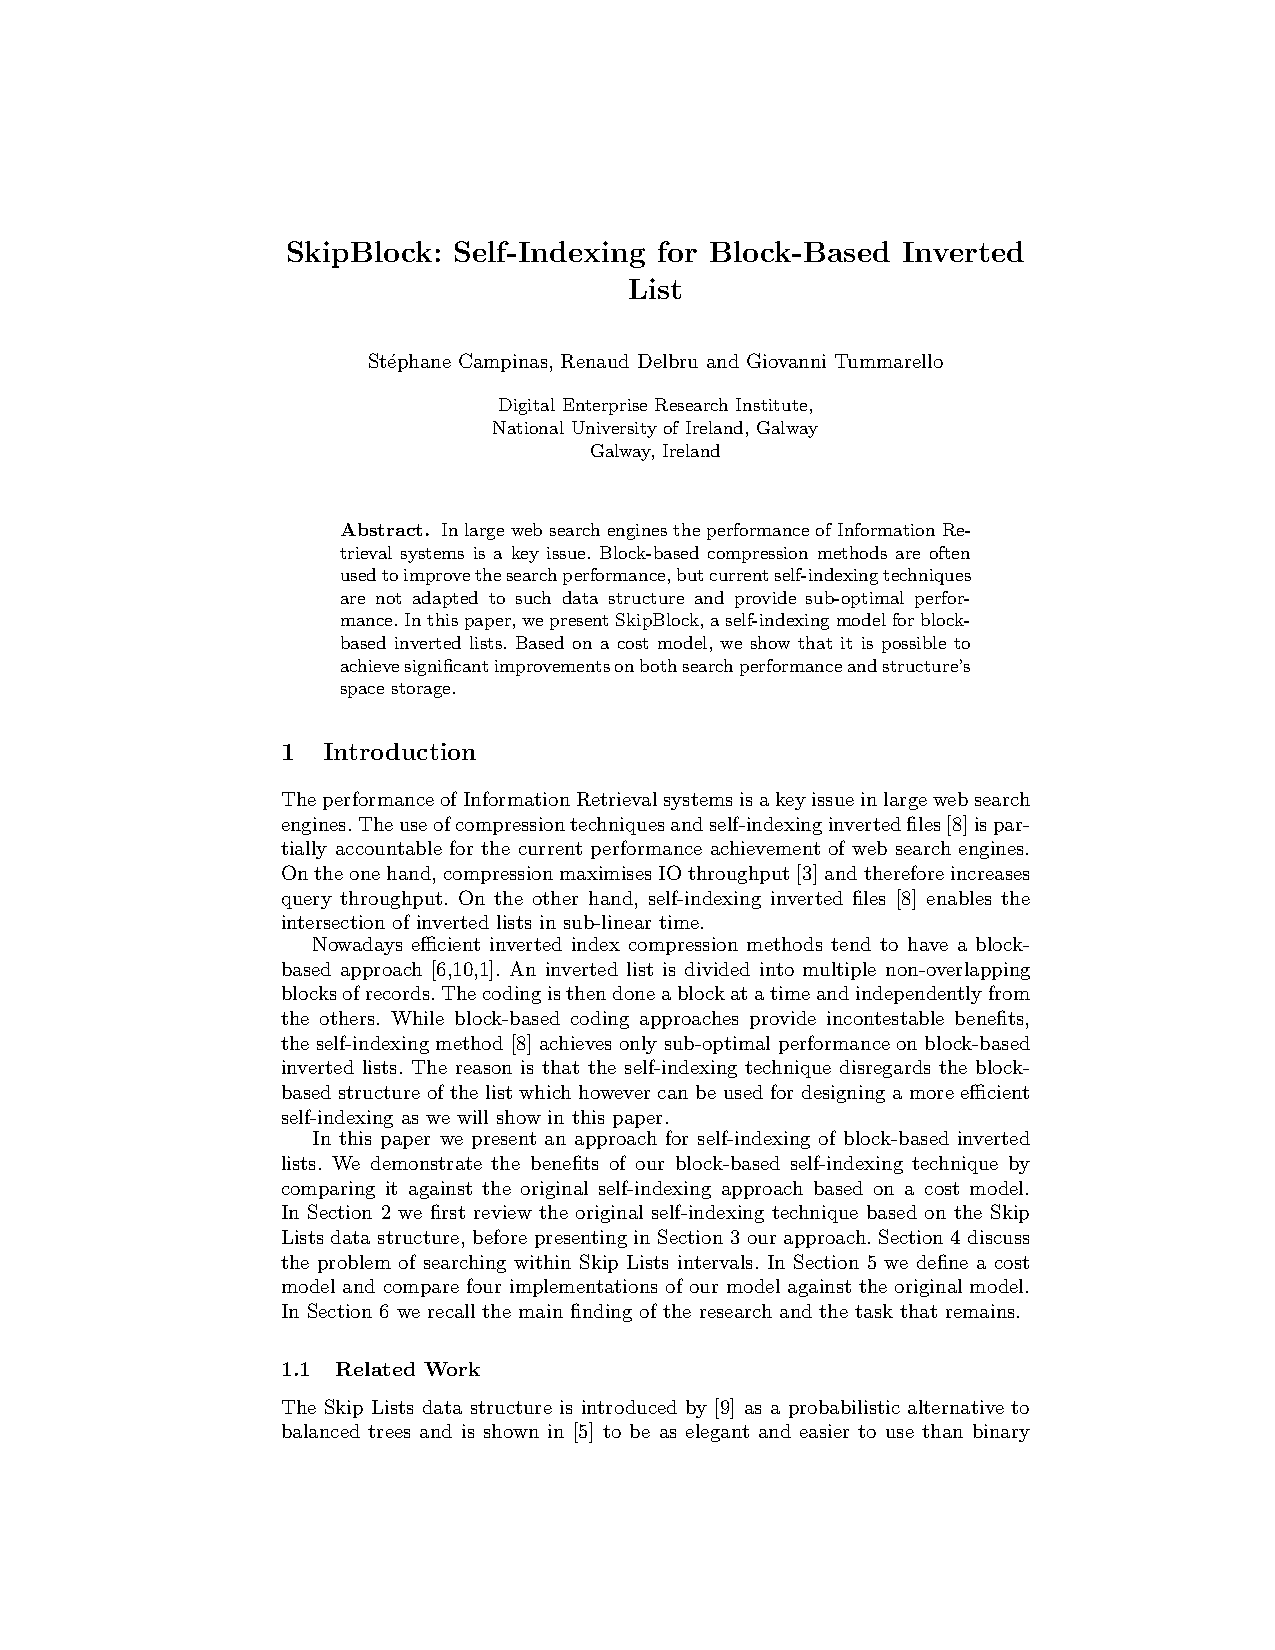
\includepdf[pages=-,delta=10 10,nup=2x1,frame=true]{skipblock-paper.pdf}
